%%%%%%%%%%%%%%%%%%%%%%%%%%%%%%%%%%%%%%%%%
% Wenneker Article
% LaTeX Template
% Version 2.0 (28/2/17)
%
% This template was downloaded from:
% http://www.LaTeXTemplates.com
%
% Authors:
% Vel (vel@LaTeXTemplates.com)
% Frits Wenneker
%
% License:
% CC BY-NC-SA 3.0 (http://creativecommons.org/licenses/by-nc-sa/3.0/)
%
%%%%%%%%%%%%%%%%%%%%%%%%%%%%%%%%%%%%%%%%%

%----------------------------------------------------------------------------------------
%	PACKAGES AND OTHER DOCUMENT CONFIGURATIONS
%----------------------------------------------------------------------------------------

\documentclass[12pt, a4paper, twocolumn]{article} % 10pt font size (11 and 12 also possible), A4 paper (letterpaper for US letter) and two column layout (remove for one column)
\usepackage{setspace}
\usepackage{multirow}
\usepackage{float}
\usepackage{hyperref}
\usepackage[USenglish,UKenglish,french,spanish,italian]{babel}

%%%%%%%%%%%%%%%%%%%%%%%%%%%%%%%%%%%%%%%%%
% Wenneker Article
% Structure Specification File
% Version 1.0 (28/2/17)
%
% This file originates from:
% http://www.LaTeXTemplates.com
%
% Authors:
% Frits Wenneker
% Vel (vel@LaTeXTemplates.com)
%
% License:
% CC BY-NC-SA 3.0 (http://creativecommons.org/licenses/by-nc-sa/3.0/)
%
%%%%%%%%%%%%%%%%%%%%%%%%%%%%%%%%%%%%%%%%%

%----------------------------------------------------------------------------------------
%	PACKAGES AND OTHER DOCUMENT CONFIGURATIONS
%----------------------------------------------------------------------------------------

\usepackage[english]{babel} % English language hyphenation

\usepackage{microtype} % Better typography

\usepackage{amsmath,amsfonts,amsthm} % Math packages for equations

\usepackage[svgnames]{xcolor} % Enabling colors by their 'svgnames'

\usepackage[hang, small, labelfont=bf, up, textfont=it]{caption} % Custom captions under/above tables and figures

\usepackage{booktabs} % Horizontal rules in tables

\usepackage{lastpage} % Used to determine the number of pages in the document (for "Page X of Total")

\usepackage{graphicx} % Required for adding images

\usepackage{enumitem} % Required for customising lists
\setlist{noitemsep} % Remove spacing between bullet/numbered list elements

\usepackage{sectsty} % Enables custom section titles
\allsectionsfont{\usefont{OT1}{phv}{b}{n}} % Change the font of all section commands (Helvetica)

%----------------------------------------------------------------------------------------
%	MARGINS AND SPACING
%----------------------------------------------------------------------------------------

\usepackage{geometry} % Required for adjusting page dimensions

\geometry{
	top=1cm, % Top margin
	bottom=1.5cm, % Bottom margin
	left=2cm, % Left margin
	right=2cm, % Right margin
	includehead, % Include space for a header
	includefoot, % Include space for a footer
	%showframe, % Uncomment to show how the type block is set on the page
}

\setlength{\columnsep}{7mm} % Column separation width

%----------------------------------------------------------------------------------------
%	FONTS
%----------------------------------------------------------------------------------------

\usepackage[T1]{fontenc} % Output font encoding for international characters
\usepackage[utf8]{inputenc} % Required for inputting international characters

\usepackage{XCharter} % Use the XCharter font

%----------------------------------------------------------------------------------------
%	HEADERS AND FOOTERS
%----------------------------------------------------------------------------------------

\usepackage{fancyhdr} % Needed to define custom headers/footers
\pagestyle{fancy} % Enables the custom headers/footers

\renewcommand{\headrulewidth}{0.0pt} % No header rule
\renewcommand{\footrulewidth}{0.4pt} % Thin footer rule

\renewcommand{\sectionmark}[1]{\markboth{#1}{}} % Removes the section number from the header when \leftmark is used

%\nouppercase\leftmark % Add this to one of the lines below if you want a section title in the header/footer

% Headers
\lhead{} % Left header
\chead{\textit{\thetitle}} % Center header - currently printing the article title
\rhead{} % Right header

% Footers
\lfoot{} % Left footer
\cfoot{} % Center footer
\rfoot{\footnotesize Page \thepage\ of \pageref{LastPage}} % Right footer, "Page 1 of 2"

\fancypagestyle{firstpage}{ % Page style for the first page with the title
	\fancyhf{}
	\renewcommand{\footrulewidth}{0pt} % Suppress footer rule
}

%----------------------------------------------------------------------------------------
%	TITLE SECTION
%----------------------------------------------------------------------------------------

\newcommand{\authorstyle}[1]{{\large\usefont{OT1}{phv}{b}{n}\color{DarkRed}#1}} % Authors style (Helvetica)

\newcommand{\institution}[1]{{\footnotesize\usefont{OT1}{phv}{m}{sl}\color{Black}#1}} % Institutions style (Helvetica)

\usepackage{titling} % Allows custom title configuration

\newcommand{\HorRule}{\color{DarkGoldenrod}\rule{\linewidth}{1pt}} % Defines the gold horizontal rule around the title

\pretitle{
	\vspace{-30pt} % Move the entire title section up
	\HorRule\vspace{10pt} % Horizontal rule before the title
	\fontsize{32}{36}\usefont{OT1}{phv}{b}{n}\selectfont % Helvetica
	\color{DarkRed} % Text colour for the title and author(s)
}

\posttitle{\par\vskip 15pt} % Whitespace under the title

\preauthor{} % Anything that will appear before \author is printed

\postauthor{ % Anything that will appear after \author is printed
	\vspace{10pt} % Space before the rule
	\par\HorRule % Horizontal rule after the title
	\vspace{20pt} % Space after the title section
}

%----------------------------------------------------------------------------------------
%	ABSTRACT
%----------------------------------------------------------------------------------------

\usepackage{lettrine} % Package to accentuate the first letter of the text (lettrine)
\usepackage{fix-cm}	% Fixes the height of the lettrine

\newcommand{\initial}[1]{ % Defines the command and style for the lettrine
	\lettrine[lines=3,findent=4pt,nindent=0pt]{% Lettrine takes up 3 lines, the text to the right of it is indented 4pt and further indenting of lines 2+ is stopped
		\color{DarkGoldenrod}% Lettrine colour
		{#1}% The letter
	}{}%
}

\usepackage{xstring} % Required for string manipulation

\newcommand{\lettrineabstract}[1]{
	\StrLeft{#1}{1}[\firstletter] % Capture the first letter of the abstract for the lettrine
	\initial{\firstletter}\textbf{\StrGobbleLeft{#1}{1}} % Print the abstract with the first letter as a lettrine and the rest in bold
}

%----------------------------------------------------------------------------------------
%	BIBLIOGRAPHY
%----------------------------------------------------------------------------------------

\usepackage[backend=bibtex,style=authoryear,natbib=true]{biblatex} % Use the bibtex backend with the authoryear citation style (which resembles APA)

\addbibresource{example.bib} % The filename of the bibliography

\usepackage[autostyle=true]{csquotes} % Required to generate language-dependent quotes in the bibliography
 % Specifies the document structure and loads requires packages

%----------------------------------------------------------------------------------------
%	ARTICLE INFORMATION
%----------------------------------------------------------------------------------------

\title{Climate Change: Temperature Prediction} % The article title

\author{
	Davide Abete, Fabrizio Cominetti e Agazzi Ruben % Authors
}

%----------------------------------------------------------------------------------------

\begin{document}

\selectlanguage{italian}

\maketitle % Print the title

\thispagestyle{firstpage} % Apply the page style for the first page (no headers and footers)

%----------------------------------------------------------------------------------------
%	ABSTRACT
%----------------------------------------------------------------------------------------
\tableofcontents
\bigskip
\bigskip
\bigskip
\bigskip
\bigskip
\lettrineabstract{Il progetto consiste nell'analisi di vari modelli di regressione applicati ad un dataset contenente le informazioni ambientali riferite alla temperatura globale a partire dal Gennaio 1850 al Novembre 2015.}

%----------------------------------------------------------------------------------------
%	ARTICLE CONTENTS
%----------------------------------------------------------------------------------------

\section{Introduzione}
\textit{Il cambiamento climatico è reale. La sfida è avvincente. E più a lungo aspettiamo, più difficile sarà risolvere il problema.} \cite{climatequote}
\bigskip

Il cambiamento climatico è da molti definito come 'la più grande minaccia del nostro tempo'. L'ultimo secolo si è reso protagonista di un aumento graduale e preoccupante della temperatura globale, ed oggi questo tema ha assunto rilevanza cruciale in numerosi dibattiti politici relativi al futuro del pianeta. \cite{climatepaper} %citare magari una ricerca
Scopo di questo progetto è di realizzare modelli di machine learning con il fine di prevedere le future temperature medie globali. Precisamente, saranno utilizzati modelli di regressione per prevedere la temperatura del mese successivo a quello preso in considerazione.
(Lo scopo di questo lavoro consiste nel realizzare e successivamente analizzare vari modelli di regressione con il fine di prevedere la temperatura media globale del mese successivo, sulla base dei dati rilevati durante la mensilità precedente.
Come specificato in apertura di sezione, la scelta di questo progetto è stata influenzata dal crescente interesse verso le tematiche riguardanti il cambiamento climatico, sia da un punto di vista personale che, appunto, globale.
I dati utilizzati per realizzare questo progetto sono scaricabili dalla piattaforma Kaggle al seguente indirizzo () e contengono diverse misure di temperature medie, rilevate ogni mese a partire dal Gennaio 1750 al Novembre 2015.

%------------------------------------------------

\section{Dataset}
Il dataset utilizzato è intitolato "Climate Change: Earth Surface Temperature Data". \cite{dataset} %citazione
Come precisato poco sopra, il dataset è stato ottenuto tramite la piattaforma Kaggle, sulla quale è stata resa disponibile una versione ripulita del dataset fornito dalla "Berkeley Earth", un'organizzazione non-profit indipendente specializata in temi di 'environmental data science'.
L'organizzazione Berkeley Earth definisce il problema del global warming come 'la sfida definitiva del nostro tempo' e pone l'accento sulla necessità di ottenere con urgenza dati di qualità e informazioni scientifiche di valore sul tema.
Il progetto è stato svolto principalmente tramite l'utilizzo della piattaforma Knime e, in particolari casi, dei linguaggi di programmazione Python e R.

\subsection{Descrizione del dataset}
Il dataset è composto da 3192 record e dai seguenti 9 attributi:
\begin{itemize}
	\item dt: data di rilevamento dei dati
	\item landAverageTemperature: temperatura media globale del terreno espressa in gradi Celsius.
	\item LandAverageTemperatureUncertainty: intervallo di confidenza al $95\%$ intorno alla media della temperatura globale
	\item LandMaxTemperature: media della temperatura massima globale del terreno espressa in gradi Celsius
	\item LandMaxTemperatureUncertainty:  intervallo di confidenza al $95\%$ intorno alla media della temperatura massima globale
	\item LandMinTemperature: media della temperatura minima globale del terreno espressa in gradi Celsius
	\item LandMinTemperatureUncertainty: intervallo di confidenza al $95\%$ intorno alla media della temperatura minima globale
	\item LandAndOceanAverageTemperature: temperatura media globale del terrestre e oceanica espressa in gradi Celsius.
	\item LandAndOceanAverageTemperatureUncertainty: intervallo di confidenza al $95\%$ intorno alla media della temperatura media terrestre e oceanica globale.
\end{itemize}

\subsection{Esplorazione dei dati}
Per la fase di esplorazione dei dati è stato utilizzato principalmente il nodo \textit{<<Statistics>>}, presente all'interno della piattaforma Knime \cite{knimewebsite}, attraverso il quale sono stati rilevati alcuni indici di posizione, variabilità e il numero di missing values, dei quali ne elencheremo i principali di seguito:
%\begin{tabular}{| m{5em} | m{1cm}| m{1cm} | m{1cm} |}
%\hline Colonna & Minimo & Massimo & Media & Deviazione Standard
%
%\end{tabular}
\begin{center}
\begin{tabular}{||c c c c||} 
 \hline
 Colonna  & Media & STD & Missing V. \\ [0.5ex] 
 \hline\hline
	Col. 1 &   8.3747 & 4.3813 & 12 \\
\hline\hline
	Col. 2 &   0.9385& 1.0964 & 12 \\
	\hline\hline
	Col. 3 & 14.3506 & 4.3096 & 1200 \\
	\hline\hline
	Col. 4 & 0.4798 & 0.5832 & 1200 \\
	\hline\hline
	Col. 5 &2.7436 & 4.1558 & 1200 \\
	\hline\hline
	Col. 6 & 0.4318 & 0.4458 & 1200 \\
	\hline\hline
	Col. 7 & 15.2126 & 1.2741 & 1200 \\
	\hline\hline
	Col. 8 & 0.1285 & 0.0736 & 1200 \\[0.5ex] \hline 
\end{tabular}
\end{center}

La fase di esplorazione ha permesso di identificare la variabile target che ci interessa prevedere, ovvero \textit{landAverageTemperature} del mese successivo, e le colonne restanti che fungono da attributi esplicativi.
La variabile target selezionata è di tipo numerico continuo e assume valori fra $[-2.080, 19.021]$ con una precisione di 3 cifre decimali.

\section{Pre-processing}
Durante la fase di esplorazione dei dati si è potuto osservare che molte colonne presentavano un numero di valori mancanti pari a 1200. Ciò è dovuto al fatto che per le osservazioni effettuate prima del Gennaio 1850 non sono stati rilevati tali dati di interesse. 

\subsection{Missing values}
Per risolvere questa problematica si è deciso di rimuovere i record che presentavano missing values, eliminando quindi 1200 righe e riducendo l'intervallo di tempo dei valori che, a questo punto, partono dal Gennaio 1850 invece che dal Gennaio 1750. Per eliminare le righe che presentavano missing values è stato utilizzato il nodo di Knime chiamato \textit{<<Missing Values>>}, configurato in modo tale da rimuovere i record contenenti valori mancanti.

\subsection{Data augmentation}
Per essere in grado di allenare i vari regressori è necessario il dato relativo alla temperatura media terrestre del mese successivo. Per fare questo abbiamo ordinato in modo decrescente i dati in base alla colonna contenente la data utilizzando il nodo \textit{<<Sorter>>} e in seguito abbiamo utilizzato il nodo \textit{<<Lag Column>>} per creare una nuova colonna contenente la temperatura media del mese successivo.

\subsection{Selezione delle variabili}
Per selezionare le variabili da utilizzare per l'apprendimento dei regressori è stato utilizzato un filtro di correlazione in modo da eliminare attributi ridondanti. Il valore soglia di correlazione scelto è di 0.9. Alla fine del processo di feature selection sono state tenute 6 colonne su 10. Per effettuare questa operazione sono stati utilizzati i nodi \textit{<<Linear Correlation>>} e \textit{<<Correlation Filter>>}. Alla fine del processo di \textit{Feature Selection} le variabili utilizzate per allenare i vari regressori sono dunque: 
\begin{itemize}
	\item LandAverageTemperature
	\item LandAverageTemperatureUncertainity
	\item LandMaxTemperatureUncertainity
	\item LandMinTemperatureUncertainity
\end{itemize}

\section{Modelli}
Per effettuare la previsione della temperatura media terrestre globale del mese successivo, sono stati utilizzati i seguenti modelli di regressione:
\begin{itemize}
	\item Regressione Lineare
	\item Regressione Polinomiale
	\item Random Forest
	\item XgBoost
	\item Tree Ensemble
\end{itemize}

\subsection{Regressione Lineare}
Il modello di regressione lineare consiste in una funzione lineare, che prende in ingresso le variabili esplicative, la cui risposta è il valore previsto della variabile target \cite{mlbook}. Nel nostro caso utilizziamo le variabili esplicative selezionate tramite feature selection per predire la variabile \textit{LandAverageTemperature}

\subsection{Regressione Polinomiale}
Il modello di regressione polinomiale, a differenza di quello lineare, prevede il valore della variabile target tramite una funzione polinomiale, in cui si può specificare il grado della funzione \cite{mlbook}. Nel nostro caso è stato scelta un polinomio di quarto grado.

\subsection{Random Forest}
Il modello di regression Random Forest è un tipo particolare di modello Tree Ensemble. In particolare il Random Forest, a differenza del modello Tree Ensemble, seleziona le variabili esplicative, usate per l'allenamto dei singoli alberi, in modo casuale \cite{randomforest}.

\subsection{XgBoost}
XgBoost è un implementazione di alberi di decisione con gradient boosting. Gli alberi di decisione sono aggiunti uno alla volta all'insieme di alberi, e configurati in modo da correggere gli errori di previsione degli alberi precedenti \cite{xgboost}. I vantaggi di XgBoost consistono nel fatto che l'apprendimento del modello è parallelizzabile, e quindi molto veloce; gestisce autonomamente eventuali missing values e inoltre previene l'overfitting del modello tramite \textit{Regularization}

\subsection{Tree Ensemble}
Il modello di regressione Tree Ensemble allena un insieme di alberi di regressione. Tipicamente ogni albero è allenato utilizzando un diverso set di righe e/o colonne del dataset. Il valore di un nodo foglia di un albero di decisione consiste nella media della variabile target dei record del dataset contenuti nel percorso del nodo foglia. Detto questo l'output di un modello di regressione Tree Ensemble è la media delle previsioni ottenute dai vari alberi di regressione \cite{treeensemble}.

\section{Training}
Per la fase di training dei modelli di regressione è stato utilizzato l'approccio della \textit{Cross Validation}.

\subsection{Cross Validation}
La Cross Validation consiste nel dividere i dati di training in \textit{K} "fogli". Per ogni foglio $k \in \lbrace1,..., K\rbrace$, eseguiamo l'allenamento del modello utilizzando $K-1$ fogli, ed eseguiamo il test sul foglio rimanente; inoltre viene eseguita questa operazione a rotazione, con numero di ripetizioni uguale al numero di fogli, in modo da eseguire il training e il testing utilizzando tutti i sottoinsiemi. Infine si calcola l'errore facendo una media fra gli errori riscontrati durante ogni ciclo di training-testing. \cite{mlbook} %citare libro
L'approccio della cross validation è molto utile in quanto permette di allenare e testare i vari regressori con tutti i dati presenti nel dataset.
Nel nostro caso abbiamo utilizzato 10 fogli, i vari record sono scelti tramite random sampling. Per l'implementazione della cross validation è stato creato per ogni modello un meta nodo, con all'interno un nodo x-partitioner, il quale effettua la divisione in "fogli", e un nodo x-aggregator per aggregare i vari risultati; inoltre, siccome il nodo x-aggregator non fornisce i valori intermedi di $R^{2}$ relativo ad ogni ciclo di cross validation, abbiamo inserito un nodo di tipo \textit{Python Script} per fornire in output queste informazioni mancanti.

\section{Valutazione}
Per la fase di valutazione dei vari modelli sono state prese in considerazione diverse metriche per ogni modello, come ad esempio i valori del coefficiente di determinazione e dell'errore quadratico medio. Inoltre, è stata effettuata un analisi dei residui dove possibile.

\subsection{Analisi $R^{2}$}
L'$R^{2}$, ovvero il \textit{coefficiente di determinazione}, rappresenta in percentuale la proporzione della variazione della variabile dipendente predetta utilizzando le variabili indipendenti \cite{r2}.\[R^{2} = 1 - \frac{SS_{res}}{SS_{tot}}\]
Per tutti i modelli è stata eseguita una comparazione delle varie misure di $R^{2}$ intermedie ad ogni passo della cross validation, misure poi estratte tramite uno script python che, in una fase successiva del workflow, abbiamo indirizzato e aggregato per ottenere una comparazione di tutti i modelli:
\begin{figure}[H]
  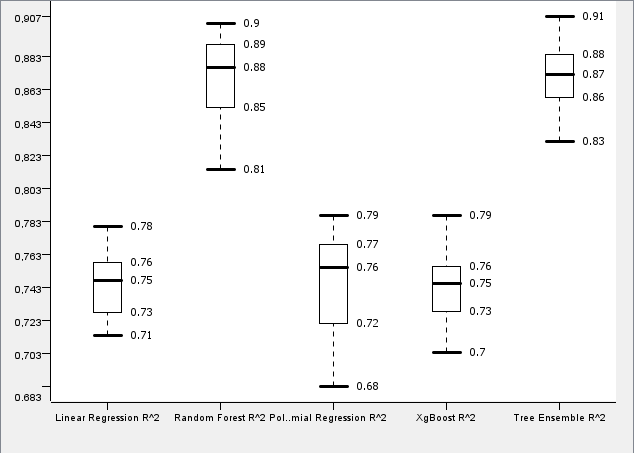
\includegraphics[scale=0.5]{./Immagini/boxplot-r2.png}
  \caption{Box plot relativo ai vari valori di $R^{2}$ di ogni ciclo della cross validation di ogni modello.}
\end{figure}
Come si può osservare dal box plot i valori migliori di $R^{2}$ sono stati ottenuti dai modelli \textit{Random Forest} e \textit{Tree Ensemble}, i quali hanno valori di $R^{2}$ compresi fra $[0,81, 0,91]$. Il fatto che questi due modelli abbiano valori simili era prevedibile, in quanto il modello \textit{Random Forest} è una variante particolare del modello \textit{Tree Ensemble}. Il valore peggiore di $R^{2}$ appartiene al modello di \textit{Regressione Polinomiale}, il quale, oltre ad avere una valore mediano pari a $0,76$, ha una grande varianza rispetto ai valori di $R^{2}$ dei vari cicli di cross validation. 

\subsection{Analisi Mean Squared Error}
Il Mean Squared Error misura la media dei quadrati degli errori presenti nelle previsioni del modello, ed è calcolato elevando al quadrato la differenza tra il valore reale y e quello predetto \cite{mse}. A fini interpretativi si precisa che i valori bassi sono i migliori.
\[MSE = \frac{1}{n} \displaystyle\sum_{i=1} ^{n} (Y_{i}-\widehat{Y_{i}})^{2}\]
Per tutti i modelli presi in considerazione è stato calcolato il valore di \textit{Mean Squared Error} ad ogni ciclo di cross-validation.
I risultati ottenuti sono i seguenti:
\begin{figure}[H]
  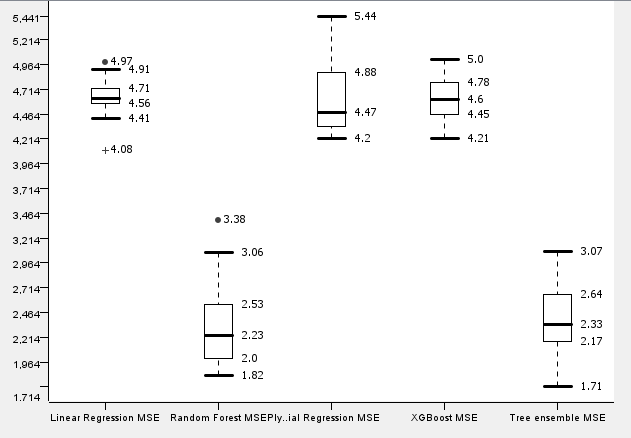
\includegraphics[scale=0.5]{./Immagini/boxplot-mse.png}
  \caption{Box plot relativo ai vari valori di \textit{MSE} di ogni ciclo della cross validation di ogni modello.}
\end{figure}
Come si può notare dal grafico i modelli con \textit{MSE} migliore, quindi più basso, sono il \textit{Tree Ensemble} ed il \textit{Random Forest}, i quali hanno valori che variano nell'intervallo $[1,71, 3,38]$. I modelli \textit{Linear Regression, Polinomial Regression e XgBoost} invece, sono quelli con \textit{MSE} peggiore, con valori che nel complesso variano nell'intervallo $[4,08 , 5,44]$.

\subsection{Analisi dei residui}
Per l'analisi della qualità dei modelli di \textit{Linear Regression e Polinomial Regression}, un passo fondamentale consiste nell'eseguire l'analisi dei residui. Questa analisi consiste nell'osservare il tipo di distribuzione assunto dai residui ottenuti nella previsione della variabile target. I residui in questione devono infatti seguire una distribuzione di tipo normale ed essere indipendenti.
Per verificare la loro distribuzione è possibile effettuare una prima analisi visiva tramite rappresentazioni grafiche, come ad esempio l'utilizzo di istogrammi, e in seguito utilizzare un test d'ipotesi, come ad esempio il test Shapiro-Wilk. Il test di Shapiro-Wilk è un test per la verifica della normalità, soprattutto per piccoli campioni, per questo motivo abbiamo selezionato un numero di record pari a 50 all'interno del nostro workflow, tramite il nodo \textit{<<Row Sampling>>}.

\subsubsection{Regressione Lineare}
In seguito ad un analisi visiva dell'istogramma relativo ai residui del modello di Regressione Lineare è possibile notare che i residui non sono distribuiti secondo una distribuzione Gaussiana:
\begin{figure}[H]
  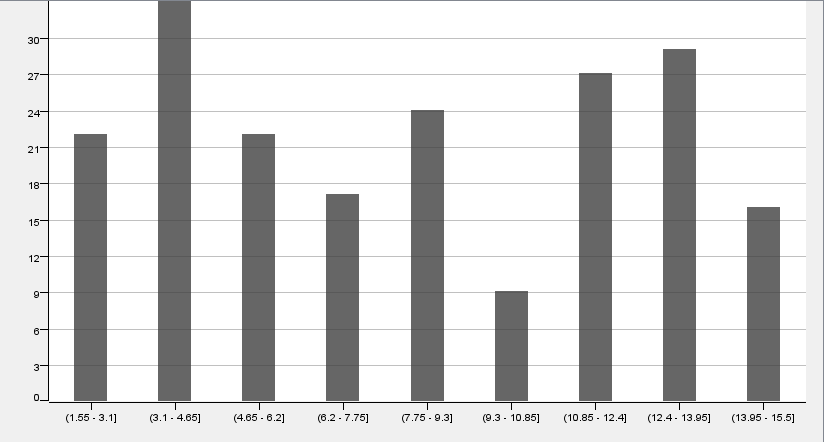
\includegraphics[scale=0.35]{./Immagini/hist-linear-regression.png}
  \caption{Istogramma relativo ai residui del modello di Regressione Lineare, si può osservare visivamente la non Normalità della distribuzione dei residui.}
\end{figure}
Per confermare l'ipotesi visiva è stato eseguito il test d'ipotesi Shapiro-Wilk, il quale ha rigettato l'ipotesi che i campioni relativi ai residui utilizzati dal test siano distribuiti seguendo una distribuzione normale.
\begin{figure}[H]
  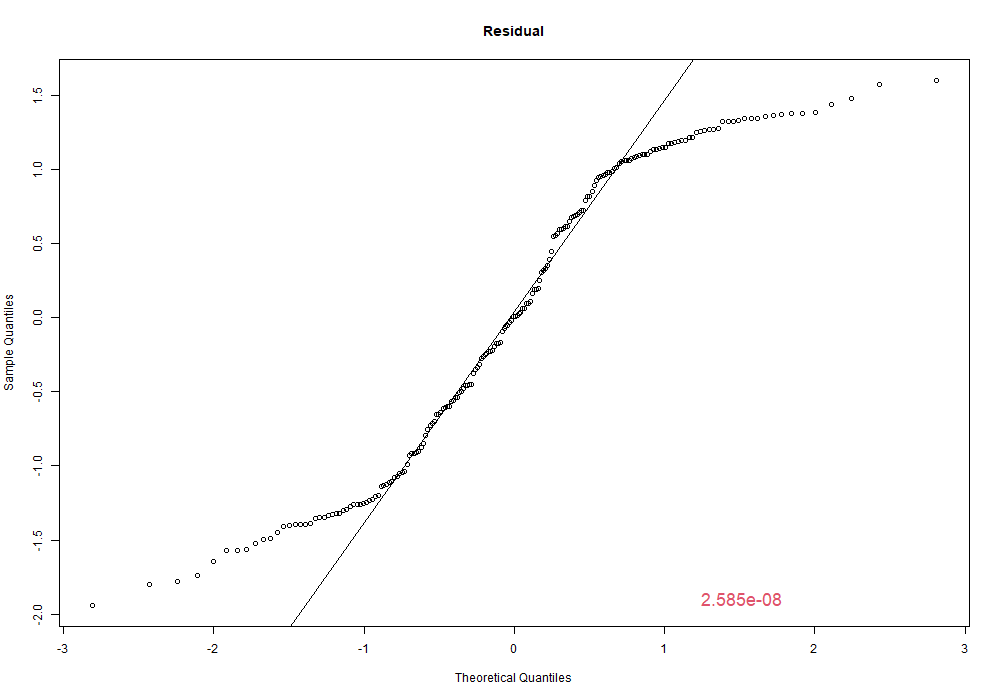
\includegraphics[scale=0.25]{./Immagini/qq-plot-linear-regression.png}
  \caption{Q Q Plot relativo ai residui del modello di Regressione Lineare}
\end{figure}
\subsubsection{Regressione Polinomiale}
Osservando visivamente la distribuzione dei residui del modello con l'aiuto di un istogramma è possibile stabilire che gli stessi residui del modello non si distribuiscano seguendo una Gaussiana:
\begin{figure}[H]
  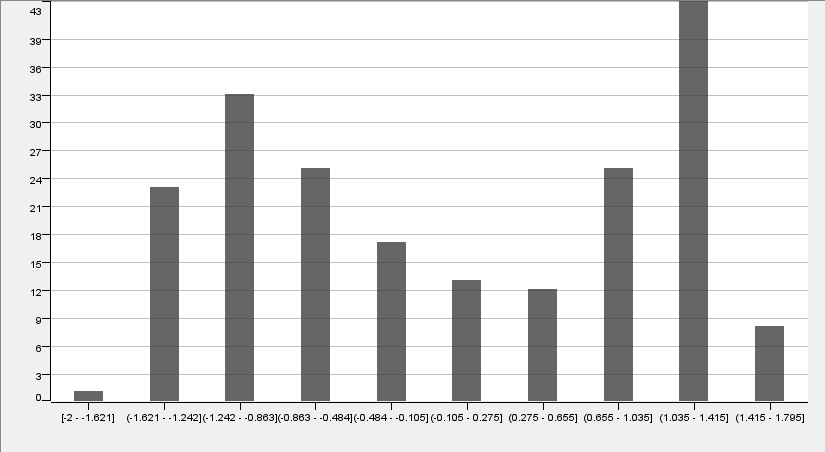
\includegraphics[scale=0.35]{./Immagini/hist-polinomial-regression.png}
  \caption{Istogramma relativo ai residui del modello di Regressione Polinomiale.}
\end{figure}
Come nel caso precedente, per confermare l'ipotesi visiva è stato eseguito il test d'ipotesi Shapiro-Wilk. Il test ha rigettato l'ipotesi che i campioni relativi ai residui utilizzati siano distribuiti seguendo una distribuzione normale.
\begin{figure}[H]
  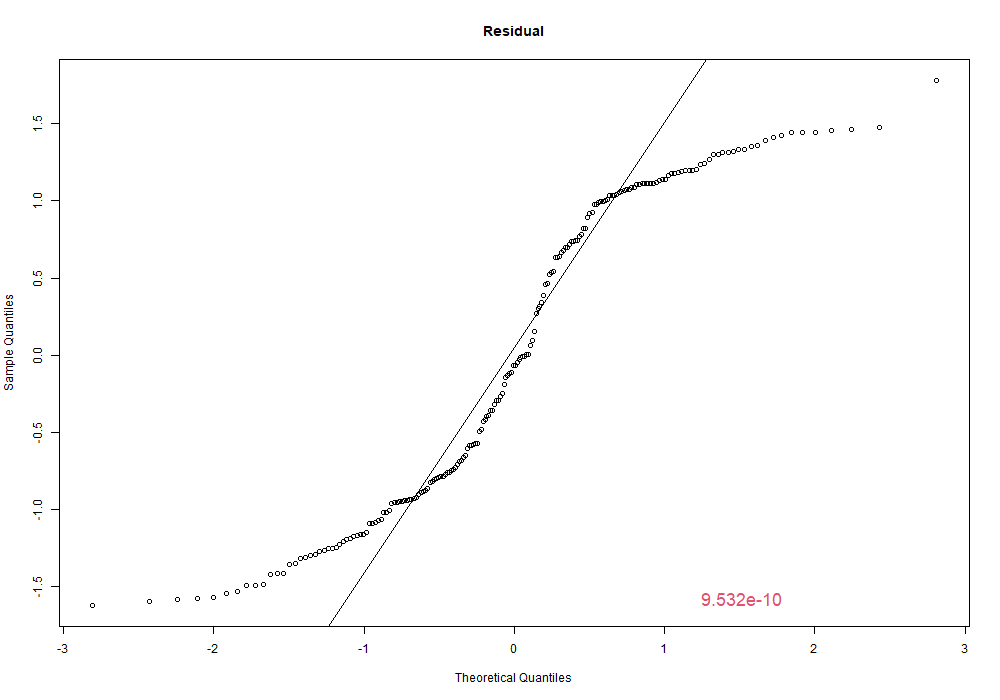
\includegraphics[scale=0.25]{./Immagini/qq-plot-polinomial-regression.png}
  \caption{Q Q Plot relativo ai residui del modello di Regressione Polinomiale.}
\end{figure}

\section{Conclusioni}
Alla luce della fase di valutazione, per raggiungere l'obiettivo di predire la temperatura media del mese successivo, si può concludere che i modelli migliori sono il \textit{Tree Ensemble ed il Random Forest}, ovvero i due modelli con $R^{2}$ maggiore e \textit{MSE} minore rispetto agli altri modelli. D'altro canto i modelli peggiori per la risoluzione di questo problema sono i modelli di \textit{Linear Regression e Polinomial Regression} che hanno ottenuto i peggiori risultati di $R^{2}$ e \textit{MSE}. Un eventuale sviluppo futuro potrebbe consistere in una migliore gestione dei valori mancanti all'interno del dataset, integrando la sorgente dati con altre sorgenti più complete, in modo da avere più dati da poter utilizzare nella fase di apprendimento dei modelli.

\printbibliography[title={Bibliografia}] %Prints bibliography

\end{document}